\documentclass{beamer-control}
\usepackage{beamer-control-singlefile}
\INCLUDEONLY{System Design Considerations}
\begin{document}
\CONCEPT{System Design Considerations}

\begin{SUMMARY}
\begin{itemize}
\item Stabilisability
\item RHP zeros and time delays
\item Bode's Integral Formula
\end{itemize}
\vfill References:
\begin{itemize}
\item \astrom{§14.1 - §14.2}
\end{itemize}
\end{SUMMARY}



\SUBCONCEPT{Stabilisability}

\begin{frame}{Stabilising unstable dynamics}
\begin{itemize}
\item One important question is when can we stabilise an unstable system, this is known as stabilisability
\item A stronger condition is when we can stabilise an unstable system with a stable controller, this is known as strong stabilisability
\item This is related to reachability, where we can find a state feedback that places closed loop eigenvalues in arbitrary positions
\item Stabilisability is slightly different --- we only have to be able to modify the unstable eigenvalues of the system
\end{itemize}
\end{frame}

\begin{frame}{Stabilisability conditions}
	\begin{itemize}
		\item A linear system with state feedback is always stabilisable if it is reachable
		\item For linear systems that are not reachable, the system is stabilisable if the unreachable part of the system is stable
		\item The Popov-Belevitch-Hautus test states that a system is reachable if and only if 
		\[\operatorname{rank}([A-\lambda I \quad B]) = n\]
		for all $\lambda\in\mathbb{C}$, and stabilisable for all $\lambda$ in the right half-plane ($\operatorname{Re} s \geq 0$)
		\item For output feedback, it is always possible to construct a stabilising controller for a system that is stabilisable and observable
	\end{itemize}
\end{frame}

\begin{frame}{Strongly stabilisability}
	\begin{itemize}
		\item A system is strongly stabilisable if it can be stabilised by a stable controller
		\item A linear system is strongly stabilisable if and only if it has an even number of real poles between every pair of real zeros in the right half-plane ($\operatorname{Re} s \geq 0$)
		\item Consider the system
		\[P(s) = \frac{(s-1)(s-5)}{(s-4)(s-6)}\]
		This system has two real zeros at $s=1$ and $s=5$ and two poles at $s=4$ and $s=6$  $\rightarrow$ not strongly stabilisable
		\item Consider the system
		\[P(s) = \frac{(s-1)(s-3)}{(s-2)^2}\]
		This system has two real zeros at $s=1$ and $s=3$ and two poles at $s=2$ $\rightarrow$ strongly stabilisable
	\end{itemize}
\end{frame}


\SUBCONCEPT{RHP zeros and time delays}

\begin{frame}{RHP zeros}
\begin{itemize}
\item Right half-plane zeros can cause limitations in closed loop performance
\item While the poles of a system depend on the system dynamics, the zeros depend on how the sensors and actuators connect to the process
\item Therefore, we may be able to redesign our system to avoid right half-plane zeros
\end{itemize}
\end{frame}

\begin{frame}{RHP zeros- Example}
	\begin{itemize}
		\item Consider the vehicle steering system
		\[P(s) = \frac{av_0s+v_0^2}{bs}\]
		where $v_0$ is the velocity of the vehicle, $a$ is the offset to reference point for the vehicle position, $b$ is the wheelbase
		\item This system has a right half-plane zero when the velocity of the vehicle is negative, which can lead to limits in the closed loop performance of the system
		\item This right half-plane zero can be removed if we instead choose to measure the location of the vehicle by the position of the center of the rear wheels, instead of the center of mass
		\item This means $a=0$ and hence our dynamics become
		\[G(s) = \frac{v_0^2}{bs}\] 
	\end{itemize}
\end{frame}


\begin{frame}{Time delays}
	\begin{itemize}
		\item Time delays are another source of limitations to closed loop performance which adds significant phase lag
		\item These delays may appear through the process, communication of information, and computation and hence cannot generally be avoided by sensor/actuator location
		\item However they have similar effects to right half-plane zeros, which can be illustrated through their Pad\'{e} approximations
	\end{itemize}
\end{frame}


\begin{frame}{Time delays- Pad\'{e} approximation}
\begin{itemize}
	\item The Pad\'{e} approximation of a time delay provides a unity gain, rational transfer function whose phase approximates the time delay
	\item The first and second order Pad\'{e} approximations are
	\[G_1(s)=\frac{1-s\tau/2}{1+s\tau/2}, \quad G_2(s)=\frac{1-\tau s/2 + \tau^2 s^2/12}{1+\tau s/2 + \tau^2 s^2/12}\]
	\item The first order approximation has a right half-plane at $s=2/\tau$ and the second order approximation has a complex conjugate pair of right half-plane zeros at $s=(3\pm i\sqrt{3})/\tau$
\end{itemize}
\end{frame}


\SUBCONCEPT{Bode's Integral Formula}

\begin{frame}{Limits of improvement}
\begin{itemize}
	\item Another limitation to controller design is that it is not possible to uniformly improve certain closed loop performance characteristics
	\item Recall the sensitivity function $S$ that attenuates disturbances of frequency $\omega$ if $|S(i\omega)|<1$ and amplifies disturbances if $|S(i\omega)|>1$
	\item The sensitivity function cannot be made small over a wide frequency range
	\item Bode's Integral Formula is a conserved quantity that implies that reducing the sensitivity at one frequency increases it at another
	\item Control design is always a compromise
\end{itemize}
\end{frame}


\begin{frame}{The integral formula}
	\begin{itemize}
		\item Let $S(s)$ be the sensitivity function of an internally stable closed loop system with loop transfer function $L(s)$, assume that $sL(s)$ goes to zero as $s\rightarrow \infty$ then Bode's Integral Formula says
		\[\int^\infty_0 \log |S(i\omega)|\, \mathrm{d}\omega  = \int^\infty_0 \log \frac{1}{|1+L(i\omega)|}\, \mathrm{d}\omega = \pi \sum p_k\]
		where $p_k$ are the right half-plane poles of $L(s)$
		\item This integral is therefore constant and can be regarded as a conservation law
	\end{itemize}
\end{frame}


\begin{frame}{Waterbed effect}
	\begin{itemize}
		\item Bode's Integral Formula tells us that if we design a controller that decreases the effect of disturbances for some frequencies, it will increase the effect for other frequencies
		\item This is known as the waterbed effect
		\item Systems with open loop right half-plane poles have larger overall sensitivity and so the effect is more severe
		\begin{figure}
			\centering
			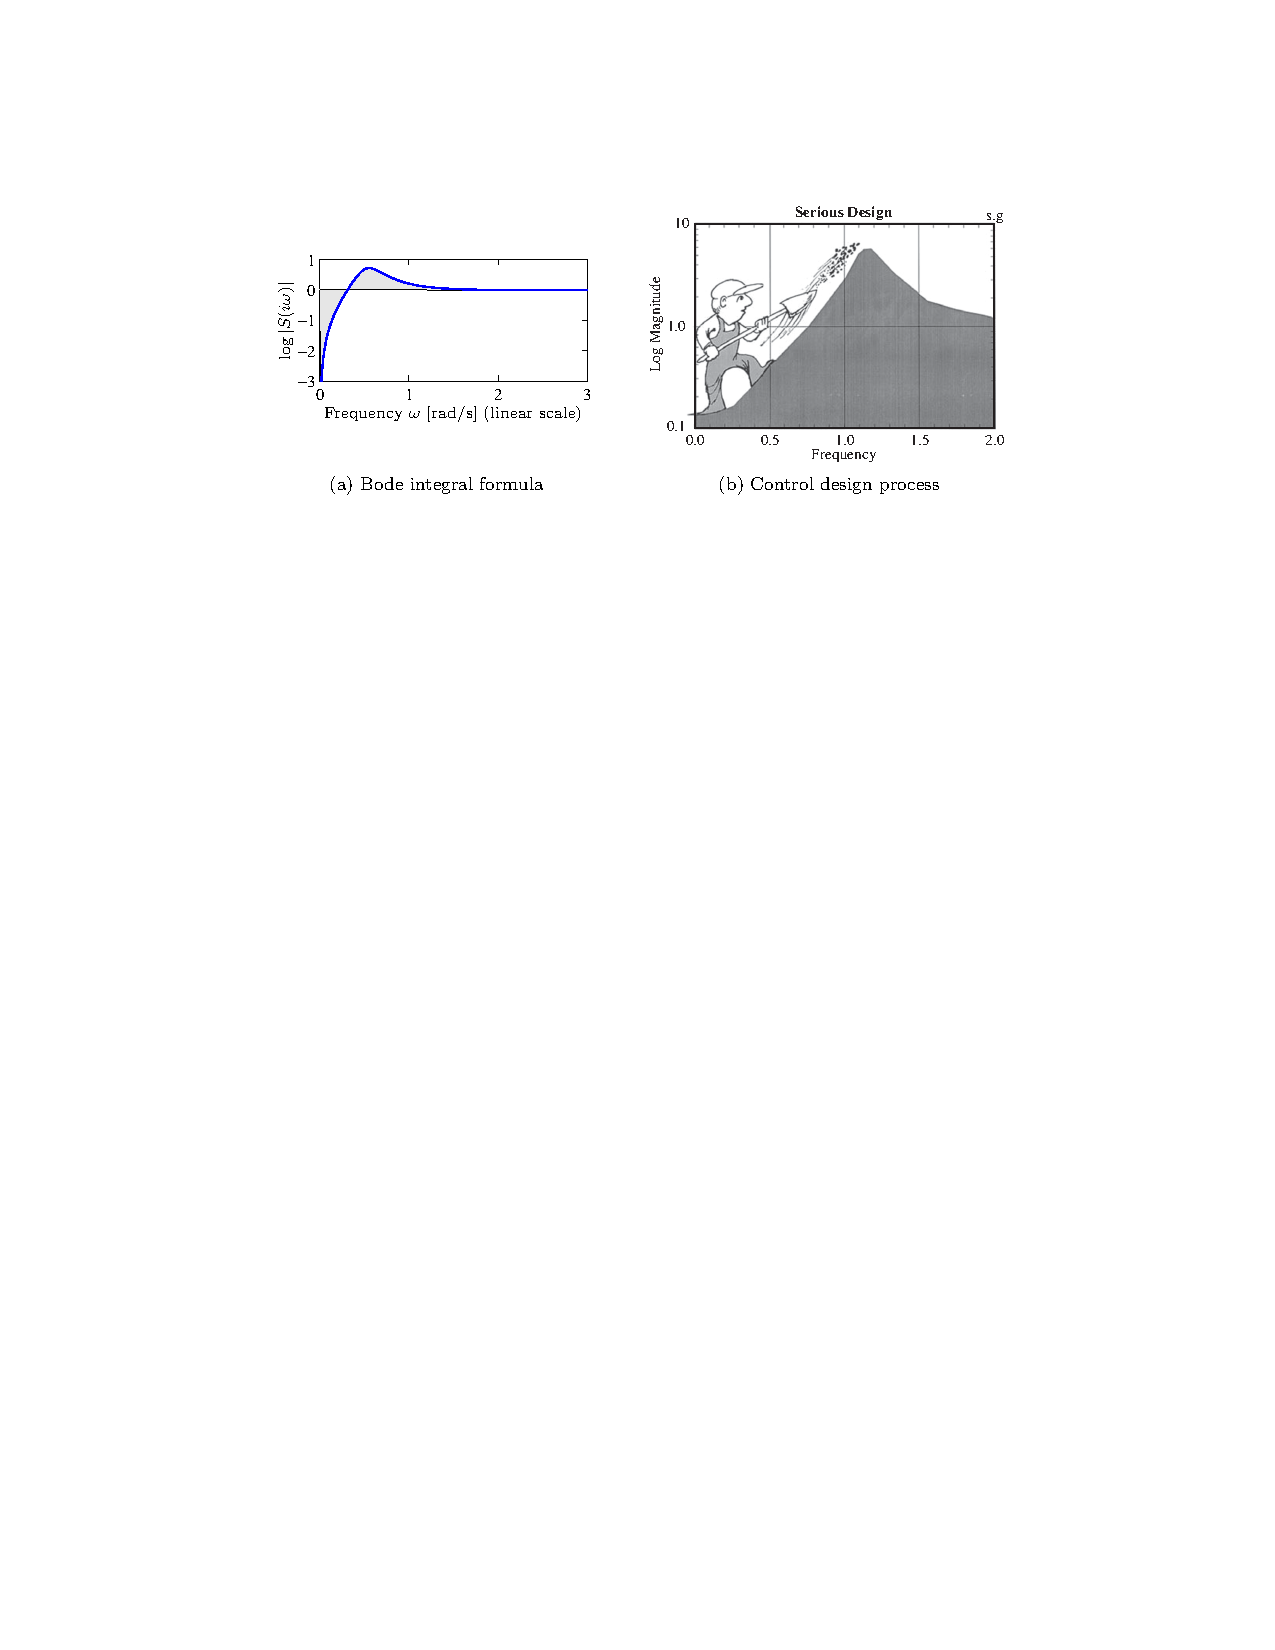
\includegraphics[width=10cm]{figure14.2}\\
			\vspace{-0.2cm}
			\textbf{Figure 14.2:} Interpretation of the waterbed effect.
		\end{figure}
	\end{itemize}
\end{frame}


\SUMMARYFRAME
\FINALE

\end{document}
